
% This LaTeX was auto-generated from an M-file by MATLAB.
% To make changes, update the M-file and republish this document.

%%% \documentclass{article}
%%% \usepackage{graphicx}
%%% \usepackage{color}

%%% \sloppy
%%% \definecolor{lightgray}{gray}{0.5}
\setlength{\parindent}{0pt}

%%% \begin{document}

    
    
\subsubsection*{Contents}

\begin{itemize}
\setlength{\itemsep}{-1ex}
   \item Calibrations Curve Computing
   \item Generate sample data
   \item Call algorithm
   \item Display results
   \item Interpolate values
   \item Plot results
\end{itemize}
\begin{lstlisting}[style=mcode]
close all
\end{lstlisting}


\subsubsection*{Calibrations Curve Computing}

\begin{par}
Example for algorithm CCC.
\end{par} \vspace{1em}
\begin{par}
Calibration Curves Computing is a software for the evaluation of instrument calibration curves
\end{par} \vspace{1em}


\subsubsection*{Generate sample data}

\begin{par}
An dependence of amplitude error (Volts, ppm) on signal frequency (Hz) of an ADC was measured and uncertainties of measurement was estimated. The uncertainty of frequency can be considered as negligible.
\end{par} \vspace{1em}
\begin{lstlisting}[style=mcode]
%3.7+12.*x+3.*x.^2
f = [10 1e2 1e3 1e4 1e5];
err = [19.700 32.700 69.700 90.700 148.700];
err_unc = [4 10 13 20 33];
\end{lstlisting}
\begin{par}
Set independent and dependent variables for \lstinline{CCC} algorithm. Lets operate in semi logarithm space for easy plotting.
\end{par} \vspace{1em}
\begin{lstlisting}[style=mcode]
DI = [];
DI.x.v = log10(f);
DI.x.u = [];
DI.y.v = err;
DI.y.u = err_unc;
\end{lstlisting}
\begin{par}
Suppose the ADC has quadratic dependence of the error on the signal frequency.
\end{par} \vspace{1em}
\begin{lstlisting}[style=mcode]
DI.exponents.v = [0 1 2];
\end{lstlisting}


\subsubsection*{Call algorithm}

\begin{par}
Use QWTB to apply algorithm \lstinline{CCC} to data \lstinline{DI}.
\end{par} \vspace{1em}
\begin{lstlisting}[style=mcode]
DO = qwtb('CCC', DI);
\end{lstlisting}

        \begin{lstlisting}[style=output]
QWTB: no uncertainty calculation
QWTB: CCC wrapper: model was set by CCC wrapper to a value `Model 2a`.
\end{lstlisting} \color{black}
    

\subsubsection*{Display results}

\begin{par}
Results is
\end{par} \vspace{1em}
\begin{lstlisting}[style=mcode]
disp(['offset          : ' num2str(DO.coefs.v(1)) ' +- ' num2str(DO.coefs.u(1))])
disp(['linear coeff.   : ' num2str(DO.coefs.v(2)) ' +- ' num2str(DO.coefs.u(2))])
disp(['quadratic coeff.: ' num2str(DO.coefs.v(3)) ' +- ' num2str(DO.coefs.u(3))])
\end{lstlisting}

        \begin{lstlisting}[style=output]
offset          : 12.6828 +- 16.9884
linear coeff.   : 1.9434 +- 19.1198
quadratic coeff.: 4.9055 +- 3.9754
\end{lstlisting} \color{black}
    

\subsubsection*{Interpolate values}

\begin{par}
Interpolate fitted polynom at values \lstinline{t}.
\end{par} \vspace{1em}
\begin{lstlisting}[style=mcode]
t = [0:0.1:6];
ty = DO.func.v(t, DO.coefs.v);
\end{lstlisting}
\begin{par}
Calculate uncertainties of interpolated values (\lstinline{S} is sensitivity matrix, \lstinline{CC} is covariance matrix of coefficients, \lstinline{CT} is covariance matrix of interpolated values, \lstinline{uty} is uncertainty of interpolated values).
\end{par} \vspace{1em}
\begin{lstlisting}[style=mcode]
for i = 1:length(t);
        S = t(i).^DI.exponents.v;
        CC = diag(DO.coefs.u,0)*DO.coefs.c*diag(DO.coefs.u,0);
        CT(i)=S*CC*S';
end
uty=CT.^0.5;
\end{lstlisting}


\subsubsection*{Plot results}

\begin{lstlisting}[style=mcode]
hold on
errorbar(DI.x.v, DI.y.v, DI.y.u, 'xb')
errorbar(DI.x.v, DO.yhat.v, DO.yhat.u, 'og')
plot(t, ty, '-r');
plot(t, ty + uty, '-r');
plot(t, ty - uty, '-r');
xlabel('log(f)')
ylabel('error of amplitude')
legend('original data','fitted values','interpolated values', 'uncer. of int. val.','location','southeast')
hold off
\end{lstlisting}

\begin{center}
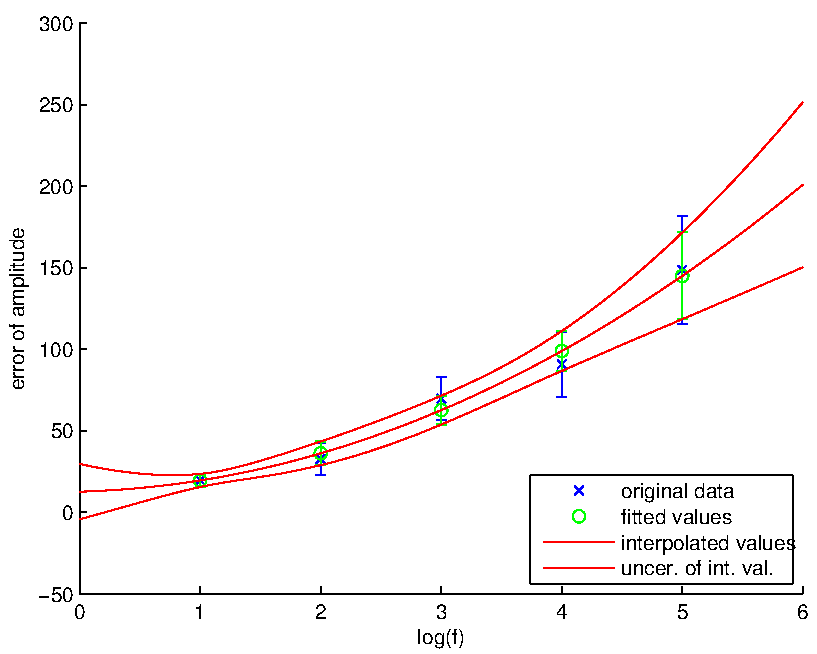
\includegraphics[width=0.7\textwidth]{algs_examples_published/CCC_alg_example_01.pdf}
\end{center}



%%% \end{document}
    
